\documentclass[aspectratio=169,12pt]{beamer}
\usepackage[utf8]{inputenc}
\usepackage[english]{babel}
\usepackage{wrapfig}
%\usepackage{siunitx}

\usepackage{multicol}
\usepackage{mathtools}

\usepackage[normalem]{ulem}

\pagestyle{empty}

\usepackage{pgf,tikz}
\usetikzlibrary{matrix}
\usetikzlibrary{arrows}

%\usepackage{wrapfig}
\mode<presentation>
\usefonttheme{professionalfonts}
\usetheme{Darmstadt}
\usecolortheme{orchid}
\useoutertheme{default}
\setbeamertemplate{headline}{}

\renewcommand{\baselinestretch}{1.1}

%gets rid of bottom navigation bars
\setbeamertemplate{footline}[page number]

%gets rid of navigation symbols
\setbeamertemplate{navigation symbols}{}

%\frameframe{none} % No default frame

%\setlength{\framewidth}{8.7in} \setlength{\frameheight}{7.2in}

\parindent 0pt
\setlength{\parskip} {1ex plus 0.5ex minus 0.2ex}


%\usepackage[bbgreekl]{mathbbol}
\usepackage{amsfonts}

%\DeclareSymbolFontAlphabet{\mathbb}{AMSb}
%\DeclareSymbolFontAlphabet{\mathbbl}{bbold}

\newcommand{\Sym}{{\mathcal S}}
\DeclareMathOperator{\Aut}{Aut}
\DeclareMathOperator{\Tr}{Tr}
\DeclareMathOperator{\trace}{Trace}
\DeclareMathOperator{\range}{range}
\DeclareMathOperator{\rank}{rank}

\usepackage{breqn}
\usepackage{multicol}
\usepackage{colortbl}
\usepackage{lmodern}
\usepackage{tabularx}
\usepackage{multirow}
\usepackage{amssymb}
\usepackage{amsmath}
\usepackage{stmaryrd}
\usepackage{color}
\usepackage{graphicx}
\graphicspath{ {img/} }
\usepackage{hyperref}

\input{epsf}
\title{Introducción}
\author{}

\DeclareMathOperator{\Hom}{Hom}
\DeclareMathOperator{\sing}{sing}

\DeclareMathOperator{\chara}{char}
\DeclareMathOperator{\Jacob}{Jacob}
\DeclareMathOperator{\Sing}{Sing}
\newcommand{\fracNoLine}[2]{\genfrac{}{}{}{0pt}{#1}{#2}}

%\beamerdefaultoverlayspecification{<+->}

\begin{document}

\newtheorem{prop}{Proposici\'on}
\newtheorem{algo}[prop]{Algorithm}
\newtheorem{teor}[prop]{Theorem}
\newtheorem{lema}[prop]{Lemma}
\newtheorem{coro}[prop]{Corollary}
\newtheorem{defi}[prop]{Definition}

\newcommand{\ideal}[1]{{\left\langle{#1}\right\rangle}}
\newcommand{\demo}{\textbf {Demostraci\'on. }}
\newcommand{\obse}{\textbf {Observaci\'on. }}
\newcommand{\Input}{\textbf {Input: }}
\newcommand{\Output}{\textbf {Output: }}
\newcommand{\Examp}{\textbf {Ejemplo }}
\newcommand{\Examps}{\textbf {Ejemplos }}

\newcommand{\kk}{{\mathbbl k}}
\newcommand{\V}{{\mathbf V}}
\newcommand{\I}{{\mathbf I}}
\newcommand{\PP}{{\tilde P}}
\newcommand{\QQ}{{\tilde Q}}

\newcommand{\F}{{\mathbb F}}
\newcommand{\Q}{{\mathbb Q}}
\newcommand{\N}{{\mathbb N}}
\newcommand{\R}{{\mathbb R}}
\newcommand{\Z}{{\mathbb Z}}
\newcommand{\CC}{{\mathbb C}}
\newcommand{\eLL}{{\mathcal L}}



\newcommand{\MinAss}{\textrm {MinAss}}
\newcommand{\Ass}{\textrm {Ass}}
\newcommand{\mcm}{\textrm {mcm}}
\newcommand{\mcd}{\textrm {mcd}}
%\newcommand{\mod}{\textrm { mod }}
\newcommand{\lt}{\textrm {lt}}
\newcommand{\Lt}{\textrm {Lt}}
\newcommand{\lp}{\textrm {lp}}
\newcommand{\lc}{\textrm {lc}}
\newcommand{\lm}{\textrm {lm}}
\newcommand{\barra}{\ /\ }
\newcommand{\multideg}{\textrm {multideg}}

\newcommand{\sep}{\textrm {sep}}
\newcommand{\Syz}{\textrm {Syz}}
\newcommand{\n}{\~n}
\newcommand{\cG}{\textrm {cG}}
\newcommand{\dG}{\textrm {dG}}
\newcommand{\nG}{\textrm {nG}}
\newcommand{\CE}{\textrm {CE}}
\newcommand{\CG}{\textrm {CG}}
\newcommand{\CF}{\textrm {CF}}
\newcommand{\DG}{\textrm {DG}}
\renewcommand{\NG}{\textrm {NG}}

\newcommand{\p}{{\boldsymbol{p}}}
\newcommand{\q}{{\boldsymbol{q}}}

\newcommand{\X}{{\boldsymbol{X}}}
\newcommand{\x}{{\boldsymbol{x}}}
\renewcommand{\u}{{\boldsymbol{u}}}
\renewcommand{\t}{{\boldsymbol{t}}}
\renewcommand{\a}{{\boldsymbol{a}}}
\renewcommand{\b}{{\boldsymbol{b}}}
\renewcommand{\c}{{\boldsymbol{c}}}

%Titulos en espa�ol
%\renewcommand{\chaptername}{Cap\'{\i}tulo}
%\renewcommand{\bibname}{Bibliograf\'{\i}a}

\newcommand{\kring}{\kk[\x]}
\newcommand{\kRing}{\kk[X]}
\newcommand{\qring}{\Q[\x]}

%\renewcommand\itemindent{-10pt}
%\renewcommand{\theenumi}{\arabic{enumi}}
%\renewcommand{\labelenumi}{\Alph{enumi}}

\definecolor{issac}{rgb}{1.00,0.00,0.00}
%------------------------------------------------------------------

\begin{frame}

 \begin{center}

\Large\textbf{Laboratorio de Datos} \\
\large\textbf{Información general}
%\vspace{0.5cm}

% \textit{Santiago Laplagne} \\
%slaplagn@dm.uba.ar \\


%\vspace{0.5cm}
%{\small Trabajo en progreso en conjunto con \emph{Jose Capco} (Universit\"at Innsbruck) y \emph{Claus Scheiderer} %(Universit\"at Konstanz).} \\

\vspace{1cm}
Primer Cuatrimestre 2024 \\ Turnos tarde y noche

\vspace{1cm}
 
 
 {\small Facultad de Ciencias Exactas y Naturales, UBA}
 \end{center}


\end{frame}

%------------------------------------------------------------------

\begin{frame}
\frametitle{Docentes}

{\large Turno tarde}

\begin{itemize}
\item Darío Elías (ayudante de primera)
\item Nazareno Fallace (ayudante de primera)
\item Santiago Laplagne (profesor)
\end{itemize}

{\large Turno noche}

\begin{itemize}
\item Gonzalo Barrera Borla (ayudante de primera)
\item Nazareno Fallace (ayudante de primera)
\item Santiago Laplagne (profesor)
\end{itemize}

\end{frame}

%------------------------------------------------------------------
%
%\begin{frame}
%\frametitle{Modelos lineales}
%
%
%\end{frame}
%
%------------------------------------------------------------------

\begin{frame}
\frametitle{Vacantes}

\begin{itemize}
\item ¿A todos los presentes les llegó un mail confirmando la vacante?
\item Si no pueden cursar, avisen a la brevedad porque hay inscriptos en lista de espera.
\end{itemize}

\end{frame}

%------------------------------------------------------------------

\begin{frame}
\frametitle{Estructura de la materia}

\begin{itemize}
\item Teórico-práctica
\item Laboratorio 1108 (turno tarde) y laboratorio 1111 (turno noche)
\item Python
\item Para aprobar la materia es necesario:
\begin{enumerate}
\item Asistir al 80\% de las clases.
\item Trabajar en clase.
\item Aprobar 2 TPs grupales (nota mayor o igual a 4).
\item Aprobar el parcial individual (nota mayor o igual a 6).
\end{enumerate}
\item $\text{Nota final} = 0.6 \times \text{nota parcial} + 0.2 \times \text{nota TP1} + 0.2 \times \text{nota TP2} +x$, donde
$$
x = \begin{cases}
1 & \text{si el promedio de los TPs es mayor o igual a 8,} \\
0 & \text{si el promedio de los TPs es menor a 8.}
\end{cases}
$$
\end{itemize}

\end{frame}

%------------------------------------------------------------------

\begin{frame}
\frametitle{Material, información y comunicación}

\begin{itemize}
\item Campus de la materia
\item Github (https://github.com/fcen-amateur/ldd)
\item Telegram
\end{itemize}
\end{frame}

%------------------------------------------------------------------

\begin{frame}
\frametitle{Fechas importantes}

\begin{itemize}
\item Entrega del primer TP: martes 21/05
\item Entrega del segundo TP: martes 18/06
\item Parcial: viernes 14/06
\item Recuperatorio del parcial: martes 25/06
\end{itemize}

\end{frame}

%------------------------------------------------------------------

\begin{frame}
\frametitle{¿Qué es la ciencia de datos?}

\begin{itemize}
\item Se define por las preguntas que se hace: es la ciencia que usa datos para describir, explicar y predecir.
\item No se define por las técnicas: no es la ciencia que usa deep learning.
\end{itemize}

\end{frame}

%------------------------------------------------------------------

\begin{frame}
\frametitle{Taxonomía de preguntas}

\begin{itemize}
\item \textbf{Descriptiva:} Resumir características de un data set. Sin interpretación, como atributos de los datos.
\item \textbf{Exploratorias:} Buscar patrones, tendencias, relaciones entre variables. Sirve para generar hipótesis
\item \textbf{Inferenciales:} Evaluar hipotesis, respecto a un patrón encontrado en un análisis exploratorio.
\item \textbf{Predictivas:} Adivinar qué va a suceder, sin importar la causa.
\item \textbf{Causales:} ¿Cambiar una variable, cambia el valor de otra variable?
\item \textbf{Mecanísticas:} ¿Cómo ocurre?
\end{itemize}

\end{frame}

%------------------------------------------------------------------

\begin{frame}
\frametitle{Objetivos generales de la materia}

¿Cómo trabajar con datos?

\begin{itemize}
\item Organización de datos.
\item Visualización, descripción y análisis exploratorio de datos.
\item Modelado de datos (modelos explicativos y predictivos).
\end{itemize}

\end{frame}

%------------------------------------------------------------------

\begin{frame}
\frametitle{Programa}

Algunos de los temas que trataremos en esta materia, en orden cronológico, serán los siguientes:

{\scriptsize
\begin{enumerate}
\item Introudcción a Python y Numpy
\item Python: lectura de archivos con Pandas, dataframes
\item Introducción a GitHub
\item Python: elaboración de gráficos
\item Mínimos cuadrados y regresión lineal
\item Introducción al modelado: datos de entrenamiento, validación y prueba
\item Mínimos cuadrados regularizados
\item Limpieza de datos, variables categóricas, datos faltantes
\item Normalización de datos
\item Aprendizaje no supervisado: clustering
\item Valores singulares y componentes principales
\item Aplicaciones de componentes principales
\item Optimización no lineal - Método del descenso
\item Introducción a Redes neuronales
\end{enumerate}
}
\end{frame}

%------------------------------------------------------------------

\begin{frame}
\frametitle{Ejemplo: ajuste de funciones}

\begin{center}
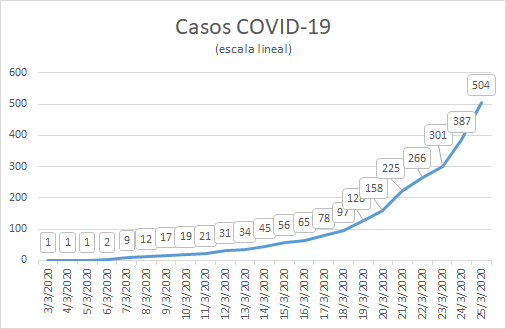
\includegraphics[scale=.35]{01-ET_lyftWoAA-gFt.png}
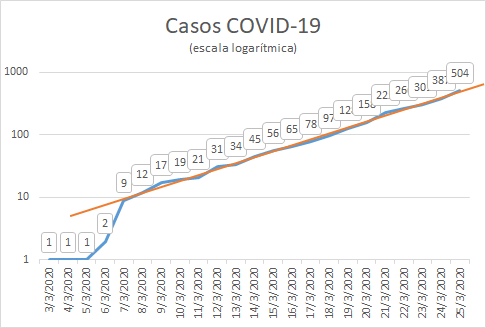
\includegraphics[scale=.35]{01-ET_l3SQXsAUhAKA.png}
\end{center}

\end{frame}


%------------------------------------------------------------------

\begin{frame}

\begin{center}
¡Largamos!

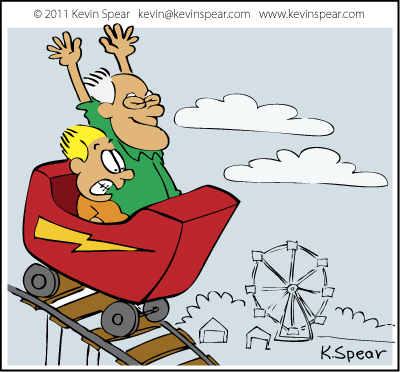
\includegraphics[scale=.5]{seatbelt.jpg}


\end{center}

\end{frame}

%------------------------------------------------------------------

\end{document}

